\documentclass{standalone}
\usepackage{ProfLycee}
\useproflyclib{ecritures}
\usepackage{tikz}
\begin{document}


\begin{tikzpicture}
  \tkzTabInit[lgt=5,espcl=2]
  {$x$ /1,
  $3\sqrt{3}x^2-120\sqrt{3}x+900\sqrt{3}$ /1,
  $V'(x)$ /1,
  $V(x)$ /2}
  {$-\infty$,$0$,$10$,$30$,$+\infty$}
  \tkzTabLine{,+,z,+,z,-,z,+,}
  \tkzTabLine{,h,t,+,z,-, t,h,}
  \tkzTabVar{-DH/,-D-/ /$0$,+/ $V(10)$,-DH/ $0$,D+/}
  \end{tikzpicture}

\end{document}


\textbf{Exprimons le volume de la boîte en fonction de $x$}

On note $\ell=BC$ la longueur d'un côté de la boîte. On a alors $\ell = 60-2x$.

Il reste à calculer l'aire du fond de la boîte, c'est-à-dire l'aire du triangle équilatéral de côté $\ell$.

On a dans le triangle rectangle $ABH$: $$AH=\sqrt{AB^2-BH^2}=\sqrt{l^2-\left(\dfrac{l}{2}\right)^2}=\sqrt{\dfrac{3}{4}l^2}=\dfrac{\sqrt{3}}{2}l$$

L'aire du triangle $ABH$ est donc $\dfrac{1}{2}\times BC \times AH = \dfrac{1}{2} \times \ell \times \dfrac{\sqrt{3}}{2}\ell = \dfrac{\sqrt{3}}{4}\ell^2=\dfrac{\sqrt{3}}{4}(60-2x)^2$.

On en déduit que le volume de la boîte est donné par $$V(x)=\mathcal{A}_{ABC}\times x=\dfrac{\sqrt{3}}{4}x(60-2x)^2$$

\textbf{Étude de la fonction $V$}:

On étudie la fonction $V$ sur l'intervalle $[0,30]$.

On a $\forall x \in \IntervalleFF{0}{30}, V(x)=\dfrac{\sqrt{3}}{4}x(60-2x)^2=\dfrac{\sqrt{3}}{4}x(4x^2-240x+3600)=\sqrt{3}x^3-60\sqrt{3}x^2+900\sqrt{3}x$.

On en déduit $\forall x \in \IntervalleFF{0}{30},  V'(x)=3\sqrt{3}x^2-120\sqrt{3}x+900\sqrt{3}$.

On calcule le déterminant de $V'$: $\Delta = (-120\sqrt{3})^2-4\times 3 \times 900\sqrt{3}=14400-10800=3600$.

On en déduit que $V'(x)$ admet deux racines: $\begin{dcases}
x_1=\dfrac{120\sqrt{3}-60\sqrt{3}}{6\sqrt{3}}=10\\
x_2=\dfrac{120\sqrt{3}+60\sqrt{3}}{6\sqrt{3}}=30
\end{dcases}$.

On en déduit le tableau de variations de $V$:

\begin{center}
\begin{tikzpicture}
\tkzTabInit[lgt=5,espcl=2]
{$x$ /1,
$3\sqrt{3}x^2-120\sqrt{3}x+900\sqrt{3}$ /1,
$V'(x)$ /1,
$V(x)$ /2}
{$-\infty$,$0$,$10$,$30$,$+\infty$}
\tkzTabLine{,+,z,+,z,-,z,+,}
\tkzTabLine{,h,t,+,z,-, t,h,}
\tkzTabVar{-DH/,-D-/ /$0$,+/ $V(10)$,-DH/ $0$,D+/}
\end{tikzpicture}
\end{center}

Le volume est donc maximal pour $x=10$ et vaut: $$V(10)=3\sqrt{3}\times 10^3-60\sqrt{3}\times 10^2+900\sqrt{3}\times 10=3000\sqrt{3}-6000\sqrt{3}+9000\sqrt{3}=6000\sqrt{3}\approx 10392~cm^3$$




\end{document}